\documentclass{beamer}
\usepackage{sdp}

\title{Списък}

\date{6 ноември 2015 г.}

\titlegraphic{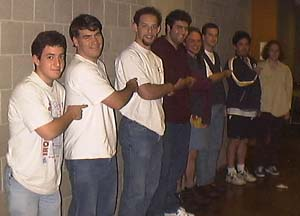
\includegraphics[height=0.35\textheight]{images/list.jpg}}

\begin{document}

\begin{frame}
  \titlepage
\end{frame}

\section{АТД списък}

\begin{frame}
  \frametitle{АТД: списък}

  Хомогенна линейна структура с последователен достъп до елементите
  \vspace{1em}

  Операции
  \vspace{0.5em}
  \begin{itemize}
  \item \tt{create()} --- създаване на празен списък
  \item \tt{empty()} --- проверка за празен списък
  \item \tt{insert(x, p)} --- включване на елемент \tt x на дадена позиция \tt p
  \item \tt{delete(p)} --- изключване на елемент на дадена позиция \tt p
  \item \tt{get(p)} --- достъп до елемент на дадена позиция \tt p
  \end{itemize}
\end{frame}

\begin{frame}
  \frametitle{Едносвързано представяне}

  \begin{center}
    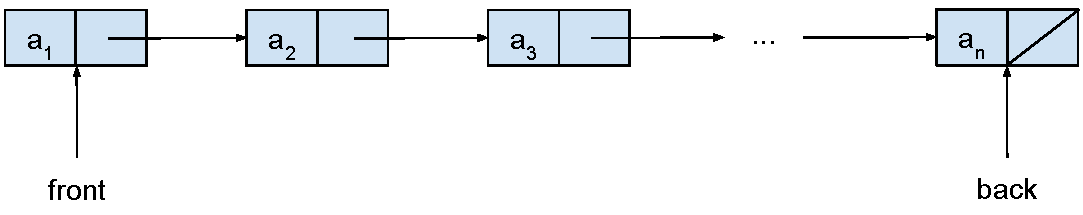
\includegraphics[width=\textwidth]{images/linked_list.pdf}
  \end{center}
\end{frame}

\begin{frame}
  \frametitle{Едносвързано циклично представяне}

  \begin{center}
    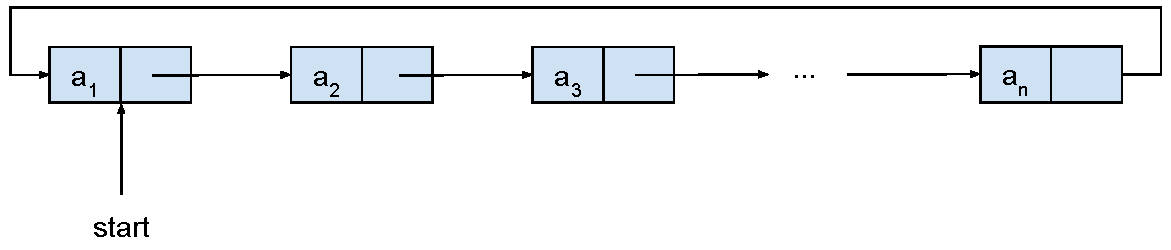
\includegraphics[width=\textwidth]{images/linked_cyclic_list.pdf}
  \end{center}
\end{frame}

\begin{frame}
  \frametitle{Двусвързано представяне}

  \begin{center}
    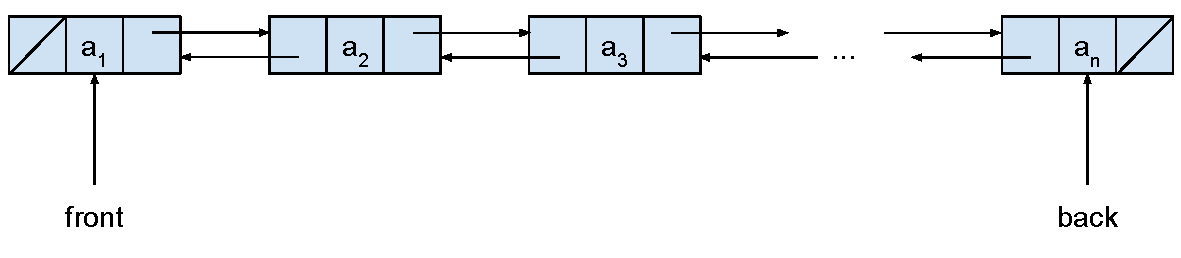
\includegraphics[width=\textwidth]{images/double_linked_list.pdf}
  \end{center}
\end{frame}

\begin{frame}
  \frametitle{Двусвързано циклично представяне}

  \begin{center}
    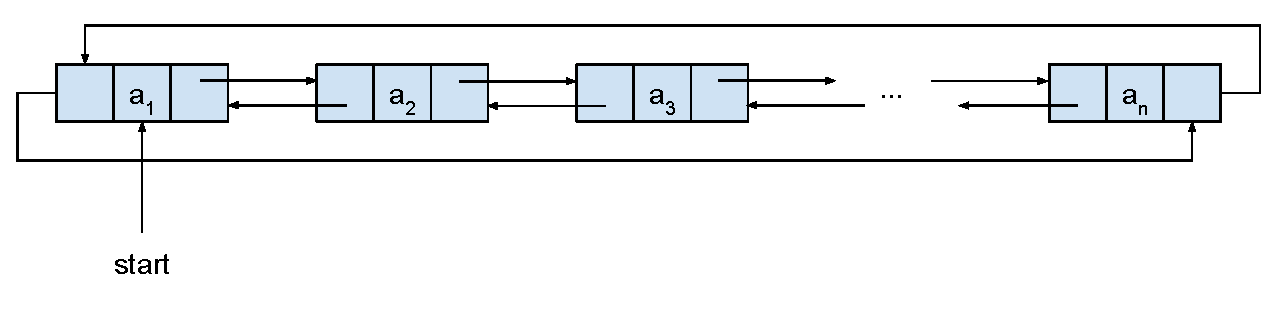
\includegraphics[width=\textwidth]{images/double_linked_cyclic_list.pdf}
  \end{center}
\end{frame}

\section{Итератори}

\begin{frame}
  \frametitle{АТД итератор}

  Абстракция на позиция, позволяваща обхождането на данни в дадена колекция
  \vspace{1em}

  Операции
  \vspace{0.5em}
  \begin{itemize}
  \item \tt{begin()} -- инициализация в началото на списъка
  \item \tt{end()} -- инициализация в края на списъка
  \item \tt{next()} -- преместване напред
  \item \tt{prev()} -- преместване назад
  \item \tt{get()} -- достъп до елемент на дадената позиция
  \item \tt{valid()} -- проверка за валидност
  \end{itemize}
\end{frame}

\begin{frame}
  \frametitle{Итератор: физическо представяне}

  \begin{itemize}
  \item при свързано представяне --- указател към двойна кутия
  \item при последователно представяне --- индекс на пореден елемент
  \end{itemize}
\end{frame}

\section{Приложения на списъци}

\begin{frame}
  \frametitle{Задачи за списъци}

  \textbf{Задача.} Да се залепи на края на даден списък втори даден списък.
  \vspace{3em}
  \pause

  \textbf{Задача.} Да се обърне реда на елементите в даден списък.
\end{frame}

\begin{frame}
  \frametitle{Сортиране чрез сливане}

  \textbf{Задача.} Да се раздели даден списък на два други с приблизително равна дължина.
  \vspace{1em}
  \pause

  \textbf{Задача.} Да се слеят два списъка, подредени във възходящ ред, в един.
  \vspace{1em}
  \pause

  \textbf{Задача.} Да се сортира дадена списък чрез сливане.
  \vspace{1em}
  \pause

  \textbf{Решение:}
  \begin{enumerate}
  \item Разделяме дадения списък на две.
  \item Всеки от получените два списъка сортираме рекурсивно.
  \item Сливаме двата сортирани списъка в един.
  \end{enumerate}
\end{frame}

\section{Функции от по-висок ред}

\begin{frame}
  \frametitle{Функции от по-висок ред за списъци}

  Нека е даден списък $l = (a_1\,a_2\,a_3\,\ldots\,a_n)$.

  \begin{itemize}[<+->]
  \item \tt{foldr} --- свиване надясно
    \begin{equation*}
      a_1 \oplus \Big(a_2 \oplus \big(\ldots \oplus (a_n \oplus \bot) \ldots\big)\Big),
    \end{equation*}
  \item \tt{foldl} --- свиване наляво
    \begin{equation*}
      \Big(\ldots\big((\bot \oplus a_1) \oplus a_2\big) \oplus \ldots\Big) \oplus a_n
    \end{equation*}
  \item \tt{map} --- изобразяване
    \begin{equation*}
      f(a_1), f(a_2), \ldots, f(a_n)
    \end{equation*}
  \item \tt{filter} --- филтриране
    \begin{equation*}
      a_{k_1}, a_{k_2}, \ldots, a_{k_m},\text{ където }\left\{
      \begin{array}{l}
        p(a_{k_i})=\mathtt{true}\text{ за }i\in\{1,\ldots,m\},\\
        p(a_k)=\mathtt{false}\text{ за }k\notin\{k_1,\ldots k_m\}
      \end{array}\right.
    \end{equation*}
  \end{itemize}
\end{frame}

\begin{frame}
  \frametitle{Задачи за функции от по-висок ред}

  \textbf{Задача.} Да се намери сумата от нечетните квадрати на числата в даден списък.
  \vspace{3em}
  \pause

  \textbf{Задача.} Да се намери произведението от най-малките положителни елементи на списък от списъци от числа.
\end{frame}

\begin{frame}
  \frametitle{Задачи за двусвързан списък}

  \textbf{Задача.} Да се провери дали даден двусвързан списък е палиндром.
\end{frame}

\end{document}
